%%%%%%%%%%%%%%%%%%%%%%%%%%%%%%%%%%%%%%%%%%%%%%%%%%%%%%
\chapter{Theoretical background}
%%%%%%%%%%%%%%%%%%%%%%%%%%%%%%%%%%%%%%%%%%%%%%%%%%%%%%

In this section I will organize and discuss the main theoretical building blocks that will be required to overcome the challenges previously identified and bring answers to the inquires this dissertation have raised. \par

\begin{figure}[h!]
    \centering
    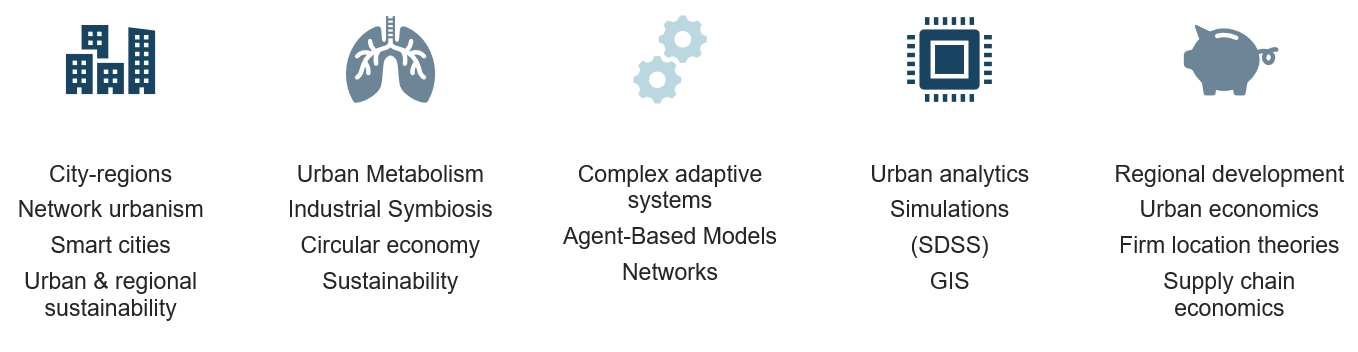
\includegraphics[width=0.8\textwidth]{sections/asset/theo.PNG}
    \caption{Theoretical background. Main research domains}
    \label{fig:theo}
\end{figure}

In order to make a substantial contribution as an interdisciplinary research and avoid falling in superficial -or wrong – analysis it would be crucial to become aware and build knowledge in different domains. Consequently, it is important to have a clear conceptual idea of the different definitions, assumptions, perspectives and biases carried within each of the fields to work with.
This dissertation will be contributing to fill gaps and build knowledge bridges between the following 3 disciplines:\par

\begin{enumerate}
    \item The goals and strategies: Sustainable development(SD)
    \item Theoretical and conceptual framework: Urban and regional science (URS)
    \item Application to real world problems: Urban \& regional planning
\end{enumerate}

In the intersection of some these big fields of research it is already possible to find advancements. However, as the outcomes of this research become clearer, also the tensions between the fields I will be trying to bridge will arise to the surface. It will become evident that the results are not contributing equally in all these fields. \par

Although, this research is borrowing from these fields simultaneously, in first place \textbf{Sustainable Development (SD)} and the contribution of \textbf{Circular Economy (CE)} as a potential strategy will be explored. Under the umbrella of circular economy, the field of industrial ecology and urban metabolism can offer theoretical frameworks to study the problems of resource efficiency. This exploration, naturally leads to 2 mainstream practices (i) \textbf{Industrial Symbiosis (IS)} and (ii) \textbf{Solid Waste Management (SWM)}. \par  

In second place, these two of how to handle resources or waste flows, partially overlaps with a well established branch of urban and regional economics. In economics and more specifically, \textbf{New Economic Geography (NEG)} has a long tradition of dealing with the location of industries, logistics and supply chains transport economics.\par

The third knowledge stream is rooted in \textbf{urban planning}. As so, in contrast with the previous ones, it starts to detach from theory and brings a specific tool-set of analytical methods to materialize the concepts highlighted before. This last domain fills the research with the necessary tools to articulate the dialogue between the first and second main areas of knowledge. \par 
This PhD will be borrowing concepts, frameworks and theory from (1) \& (2), and the outcomes will contribute to build tools and expand the knowledge of how to plan sustainable city-regions. \par















% \section{On the importance of Circular Economy}
% What is Circular Economy? Give a definition 



% Implementation worldwide still in early stages [1] 
% Metrics and other assessment methods will play a key role in understanding [2] 
% Main aim of the CE is considered to be economic prosperity, followed by environmental quality; social equity and future generations is barely mentioned [3] 
% 7 strategies are conceptualized to implement CE in cities [4]

% [1] (Ghisellini et al, 2016)
% [2] (Blomsma & Brennan, 2017)
% [3] (Kirchherr, 2017)
% [4] (Williams, 2019)





% Urban planning contributes to simulate circular processes at different scales through a systemic approach and evoking the approaches of industrial ecology [1]
% Urban metabolism as a planning tool to identify opportunities for CE initiatives and monitoring of progress [2]
% Understanding of the spatial relationships between a city and its hinterlands and global resource networks is critical for urban policy makers [3]


% [1] (Girard et al., 2019) 
% [2] (Kalmykova & Rosado, 2015)
% [3] (Kennedy et al., 2007) 





% \begin{figure}[h!]
%     \centering
%     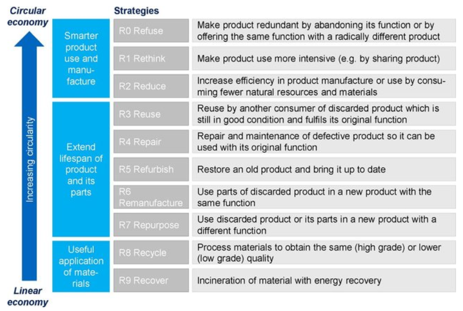
\includegraphics[width=0.7\textwidth]{sections/asset/rs.png}
%     \caption{Circular economy ladder of strategies}
%     \label{fig:badbad}
% \end{figure}




